% Options for packages loaded elsewhere
\PassOptionsToPackage{unicode}{hyperref}
\PassOptionsToPackage{hyphens}{url}
%
\documentclass[
]{article}
\usepackage{amsmath,amssymb}
\usepackage{iftex}
\ifPDFTeX
  \usepackage[T1]{fontenc}
  \usepackage[utf8]{inputenc}
  \usepackage{textcomp} % provide euro and other symbols
\else % if luatex or xetex
  \usepackage{unicode-math} % this also loads fontspec
  \defaultfontfeatures{Scale=MatchLowercase}
  \defaultfontfeatures[\rmfamily]{Ligatures=TeX,Scale=1}
\fi
\usepackage{lmodern}
\ifPDFTeX\else
  % xetex/luatex font selection
\fi
% Use upquote if available, for straight quotes in verbatim environments
\IfFileExists{upquote.sty}{\usepackage{upquote}}{}
\IfFileExists{microtype.sty}{% use microtype if available
  \usepackage[]{microtype}
  \UseMicrotypeSet[protrusion]{basicmath} % disable protrusion for tt fonts
}{}
\makeatletter
\@ifundefined{KOMAClassName}{% if non-KOMA class
  \IfFileExists{parskip.sty}{%
    \usepackage{parskip}
  }{% else
    \setlength{\parindent}{0pt}
    \setlength{\parskip}{6pt plus 2pt minus 1pt}}
}{% if KOMA class
  \KOMAoptions{parskip=half}}
\makeatother
\usepackage{xcolor}
\usepackage[margin=1in]{geometry}
\usepackage{longtable,booktabs,array}
\usepackage{calc} % for calculating minipage widths
% Correct order of tables after \paragraph or \subparagraph
\usepackage{etoolbox}
\makeatletter
\patchcmd\longtable{\par}{\if@noskipsec\mbox{}\fi\par}{}{}
\makeatother
% Allow footnotes in longtable head/foot
\IfFileExists{footnotehyper.sty}{\usepackage{footnotehyper}}{\usepackage{footnote}}
\makesavenoteenv{longtable}
\usepackage{graphicx}
\makeatletter
\def\maxwidth{\ifdim\Gin@nat@width>\linewidth\linewidth\else\Gin@nat@width\fi}
\def\maxheight{\ifdim\Gin@nat@height>\textheight\textheight\else\Gin@nat@height\fi}
\makeatother
% Scale images if necessary, so that they will not overflow the page
% margins by default, and it is still possible to overwrite the defaults
% using explicit options in \includegraphics[width, height, ...]{}
\setkeys{Gin}{width=\maxwidth,height=\maxheight,keepaspectratio}
% Set default figure placement to htbp
\makeatletter
\def\fps@figure{htbp}
\makeatother
\setlength{\emergencystretch}{3em} % prevent overfull lines
\providecommand{\tightlist}{%
  \setlength{\itemsep}{0pt}\setlength{\parskip}{0pt}}
\setcounter{secnumdepth}{-\maxdimen} % remove section numbering
\ifLuaTeX
  \usepackage{selnolig}  % disable illegal ligatures
\fi
\usepackage{bookmark}
\IfFileExists{xurl.sty}{\usepackage{xurl}}{} % add URL line breaks if available
\urlstyle{same}
\hypersetup{
  pdftitle={Exploratory Data Analysis: Google Play Store Apps},
  pdfauthor={Snehitha Tadapaneni, Sai Rachana Kandikattu, Amrutha Jayachandradhara, Wilona Nguyen, Pramod Krishnachari},
  hidelinks,
  pdfcreator={LaTeX via pandoc}}

\title{Exploratory Data Analysis:Google Play Store Apps}
\author{Snehitha Tadapaneni, Sai Rachana Kandikattu, Amrutha
Jayachandradhara, Wilona Nguyen, Pramod Krishnachari}
\date{2024-11-02}

\begin{document}
\maketitle

{
\setcounter{tocdepth}{2}
\tableofcontents
}
\section{\texorpdfstring{\textbf{Introduction}}{Introduction}}\label{introduction}

In the rapidly evolving smartphone landscape, Android has emerged as the
dominant mobile operating system, now powering over 2.5 billion active
devices worldwide (Brandom, 2019). This extensive user base encompasses
nearly 90\% of smartphone users engaged with Android devices. A key
aspect of this experience is the Google Play Store, which offers a
diverse range of applications that simplify various aspects of daily
life, from productivity to entertainment.

There were several factors which drove the decision to analyze the
Google Play Store dataset. First, it provides free, real-time data that
allows developers and researchers to assess user interactions without
financial barriers, making it an invaluable resource for uncovering
trends in user engagement. Second, the dataset includes important app
metrics, such as category, rating, and reviews, enabling deeper
exploration of user behavior and preferences.

Understanding these preferences is crucial for developers aiming to
create successful applications. Each interaction within the Play Store
offers critical insights into the factors that significantly influence
app popularity. This analysis will identify trends in the dataset to
enhance understanding of users. By examining variables such as app
category, update frequency, Android version compatibility, content
ratings, and the impact of positive reviews and ratings, we can
delineate the elements that drive app installations and overall
popularity. The nuanced relationships among these data points are
essential for developers seeking to create applications that resonate
with users. By detecting patterns through this analysis, we can provide
valuable insights to developers, equipping them with the information
needed to craft better apps tailored to user expectations and
preferences. This research aims to deepen our understanding of user
dynamics in an ever-evolving app ecosystem, which is critical for
fostering user engagement and satisfaction.

\section{\texorpdfstring{\textbf{Literature
Review}}{Literature Review}}\label{literature-review}

During the investigation of user interactions with mobile applications,
a range of methodologies was explored to gain an expert perspective. It
was discovered that numerous studies have been conducted to provide
insights into how users engage with apps on platforms such as the Google
Play Store.~ Initially, a comprehensive review of existing literature
was conducted to understand the dynamics of user behavior and app
engagement. Notably, the study ``Building a Quality Mobile Application:
A User-Centered Study Focusing on Design Thinking, User Experience and
Usability'' was analyzed, highlighting the importance of user-centric
design (Paula et al., 1970). This research illustrated that positive
user experiences significantly contribute to app success and retention
rates, suggesting that developers should prioritize understanding user
needs and preferences.

Expert analyses from various sources further supported the findings,
indicating that emotional responses play a crucial role in user
satisfaction. Overall, the conducted research underscores the nuanced
relationships between user interactions and app design, suggesting that
a deeper understanding of these dynamics can lead to the development of
more effective and engaging applications.

\begin{center}\rule{0.5\linewidth}{0.5pt}\end{center}

\section{\texorpdfstring{\textbf{Data
Description}}{Data Description}}\label{data-description}

The dataset used in this study is a popular collection of Google Play
Store apps, sourced from Kaggle (faisaljanjua0555, 2023). It contains
detailed information about 10,841 apps, organized across 13 variables,
with each row representing an individual app. The dataset covers a range
of app attributes, such as ratings, reviews, size, category, installs,
price, and content rating, providing valuable insights into the
characteristics that contribute to app popularity and user engagement.
This comprehensive data serves as a foundation for analyzing patterns in
user behavior, app performance, and trends within the mobile app
ecosystem. Below is a breakdown of each column in the Google Play Store
apps dataset:

\begin{longtable}[]{@{}
  >{\raggedright\arraybackslash}p{(\columnwidth - 2\tabcolsep) * \real{0.2778}}
  >{\raggedright\arraybackslash}p{(\columnwidth - 2\tabcolsep) * \real{0.7222}}@{}}
\toprule\noalign{}
\begin{minipage}[b]{\linewidth}\raggedright
Variable
\end{minipage} & \begin{minipage}[b]{\linewidth}\raggedright
Description
\end{minipage} \\
\midrule\noalign{}
\endhead
\bottomrule\noalign{}
\endlastfoot
App & The name of the app. \\
Category & The app category (e.g., ART\_AND\_DESIGN, BUSINESS). \\
Rating & The user rating of the app on a scale from 1 to 5 (float). \\
Reviews & The number of user reviews for the app, stored as text and
needs conversion to numeric for analysis. \\
Size & The app size (e.g., ``19M'', ``14M'', ``Varies with device''),
which may need cleaning to standardize for analysis. \\
Installs & The number of installs as a text field (e.g., ``10,000+'',
``1,000,000+''), requiring conversion to numeric. \\
Type & Whether the app is ``Free'' or ``Paid''. \\
Price & The app's price (in USD), with free apps listed as ``0'' and
paid apps with the price value in text format. \\
Content Rating & The age rating of the app (e.g., ``Everyone'',
``Teen''). \\
Genres & The genre(s) of the app, sometimes containing multiple genres
separated by semicolons. \\
Last Updated & The date when the app was last updated, stored as text
and can be converted to a date format. \\
Current Ver & The current version of the app, stored as text and might
have different formats. \\
Android Ver & The minimum Android version required to run the app, given
as text (e.g., ``4.0.3 and up''). \\
\end{longtable}

Here's a visualization of our dataset structure:
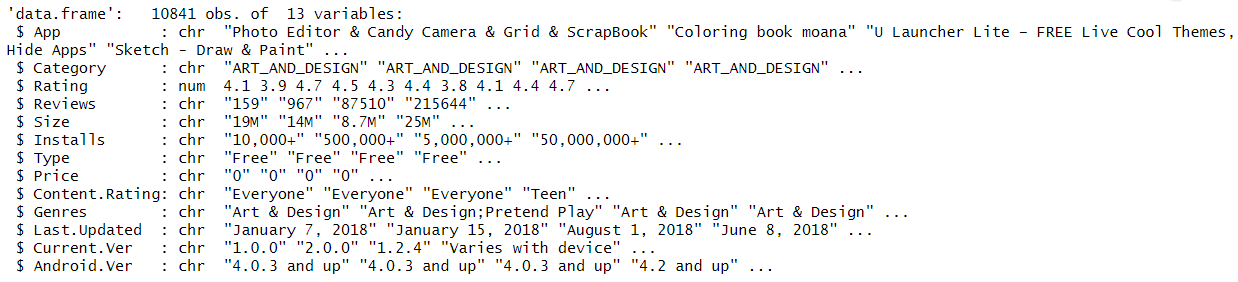
\includegraphics{data_structure.png} ---

\section{\texorpdfstring{\textbf{Data
Limitations}}{Data Limitations}}\label{data-limitations}

The Google Play Store dataset we choose provides valuable insights into
app performance and user reviews, but including few features might help
us analyse the depth and accuracy of our analysis.

Features like user engagement metrics, for example how often the user
engage with the app after installation or if he deletes the app later,
sessionlength etc would let us understand deeper and help differentiate
between one-time installs and regular users.

The dataset has several missing values, particularly in the Rating
column, which necessitates careful handling to avoid introducing bias
into the analysis. Additionally, the absence of demographic information
about users, such as age, location, or device type restricts our ability
to segment user groups or understand how various demographics interact
with different app categories (Fischer, \& Kleen 2021).

An additional aspect of the data that could have been included is the
reviews, which would have been valuable for assessing whether the
feedback is positive or negative. This information would provide further
insights into whether a higher number of reviews correlates with a
positive reception.

Further, the inclusion of data on marketing efforts, like ad spend or
whether an app was featured on the Play Store, could clarify the impact
of promotion on installs and ratings.

\paragraph{Missing records in our
Data}\label{missing-records-in-our-data}

\begin{center}\rule{0.5\linewidth}{0.5pt}\end{center}

\section{\texorpdfstring{\textbf{Exploratory Data Analysis
(EDA)}}{Exploratory Data Analysis (EDA)}}\label{exploratory-data-analysis-eda}

\subsubsection{Data Exploring}\label{data-exploring}

The dataset has several missing values, particularly in the Rating
column, which necessitates careful handling to avoid introducing bias
into the analysis. Additionally, there is no demographic information
about users, such as age, location, or device type, which restricts our
ability to segment user groups or understand how various demographics
interact with different app categories.

\subsubsection{Data Cleaning}\label{data-cleaning}

The Google Play Store dataset, as analyzed, contains missing values and
inconsistent formats across various columns. To clean and prepare this
dataset for analysis, several steps were taken to address these data
quality issues. Here is an overview of how missing records were managed
and further improvements that could be considered:

\begin{itemize}
\item
  Duplicates in App Names: Initially, there were 404 duplicated apps
  that appeared twice or even thrice. By removing these duplicates, the
  dataset was reduced from 10,841 to 9,660 unique apps. This ensures
  that only one instance of each app is considered, eliminating
  redundancy and potential skew in subsequent analysis. Total duplicates
  removed: 1,181 apps.
\item
  Price Column: The Price column contained dollar symbols (\$) that had
  to be removed for conversion to numeric format. After cleaning,
  missing values were identified in the Price column. These missing
  values were handled by removing rows where Price was NA or blank. Rows
  with missing or blank prices were dropped, as they were not relevant
  for assessing price impact on app installs.
\item
  Type Column: The Type column had one missing value, where the Type was
  NA. Since the Price was recorded as 0 for this app, it was assumed to
  be a ``Free'' app. This missing value was replaced with ``Free'' to
  maintain data consistency. This replacement decision was made based on
  logical inference, ensuring the data accurately reflects app types
  without dropping valuable records.
\item
  Size Column: The Size column had a mix of values in kilobytes (KB) and
  megabytes (MB), as well as entries labeled ``Varies with device.'' The
  latter were treated as NA and replaced with the mean size for each
  category. Apps with sizes marked as ``Varies with device'' or having
  missing sizes were assigned the average size of other apps in the same
  category. This approach allowed retention of records while maintaining
  reasonable size estimates.
\item
  Installs Column: The Installs column contained entries with symbols
  like + and commas, which were removed to convert the data into a
  numeric format. Some records had non-numeric entries or unusual
  characters, so these were cleaned systematically. A custom function
  was used to remove these symbols, ensuring all install counts were
  represented as clean, comparable integers.
\item
  Rating and Reviews Columns: The Rating column contained 1,463 missing
  values, predominantly in the ``Family'' category. Rather than dropping
  these records, the missing values were replaced with the mean rating
  of apps within the same category. This imputation method helped
  maintain category-wise data integrity. The Reviews column, initially
  in string format, was converted to integer format after addressing
  missing values. Converting to numeric allowed for statistical
  analysis, such as calculating averages or correlations with installs
  or ratings.
\item
  Last Updated: The date format in the ``Last Updated'' column was
  adjusted to an appropriate format to ensure accurate analysis.
\item
  Category and Genres: The dataset consists of 33 unique values for
  Category and 118 for Genres, meaning multiple genres fall under each
  category. Since genres are already embedded within categories,
  retaining both columns could introduce redundancy and complicate the
  analysis. This simplifies the dataset while preserving the essential
  structure needed for meaningful insights.
\item
  Current Version:~ The format of the ``Current Version'' values for
  apps varies among developers, making it difficult to achieve
  consistency across the dataset. Due to this variability, it has been
  determined that this variable will be excluded from the analysis. By
  removing the ``Current Version'' column, the dataset can maintain
  clarity and focus on more consistent and relevant attributes that
  contribute to app success.
\item
  Android Version: Although there are no missing values for the
  ``Android Version'' variable, two rows contain `NaN' entries, which
  have been removed from the dataset.
\end{itemize}

Additional Transformations done for effective analysis:

\begin{itemize}
\item
  Review Category The review category was binned to ensure that each
  category contained an approximately equal number of reviews. This
  approach enhances the validity of the comparisons, as it prevents any
  one category from dominating the analysis due to an excessive number
  of reviews. Binning allows for a more balanced representation of
  different review sentiments across categories, facilitating a clearer
  understanding of how reviews impact app success.
\item
  Install Category The install category was created based on the
  distribution of installs present in the dataset. By analyzing the
  install figures, the data was binned into meaningful segments,
  ensuring that each segment reflects a realistic range of installs.
  This method allows for a comparative analysis of how different levels
  of installs correlate with other variables, such as ratings and review
  categories.
\item
  Log Transformed Installs Log transformation of installs was utilized
  to normalize the data, making it easier to compare and analyze the
  installations across various categories. This transformation is
  particularly useful in addressing the skewness commonly present in raw
  install data, enabling a more straightforward comparison of
  distributions. By applying the log transformation, we can better
  visualize relationships and draw more reliable conclusions regarding
  app success metrics.
\item
  Update Category The update category distinguishes between ``Old
  Update'' and ``Recent Update,'' based on the update time recorded in
  the dataset. This categorization allows for the assessment of how
  recent updates may affect user perceptions and app performance. By
  classifying apps into these two groups, we can investigate the
  potential impact of frequent updates on installs and overall app
  ratings.
\end{itemize}

\subsubsection{Data Visualization}\label{data-visualization}

To illustrate the relationships between the variables, we employed
various visualization methods, including bar plots, scatter plots, heat
maps, and other techniques. The selection of these visualization methods
was based on the types of variables being plotted and their relevance to
our analysis. This approach aimed to identify which applications exhibit
the highest popularity by examining the relationships among reviews,
ratings, and installs. If a positive relationship is evident among these
metrics, we can concentrate on the relationship with installs, as it
ultimately reflects the user base for an application.

The visualizations we have chosen include:

\begin{enumerate}
\def\labelenumi{\arabic{enumi}.}
\tightlist
\item
  Installs and Price
\item
  Ratings and Days since last update
\item
  Installs and Update Category and Content Rating
\item
  Installs and size
\item
  Installs and Rating
\item
  Ratings and Review Category
\item
  Installs and Review Category
\item
  Top 5 Categories with Highest Installs
\end{enumerate}

These visualizations are designed to provide insights into the factors
influencing app success on the Google Play Store.

\textbf{Figure 1}. Scatterplot for Price and Installs

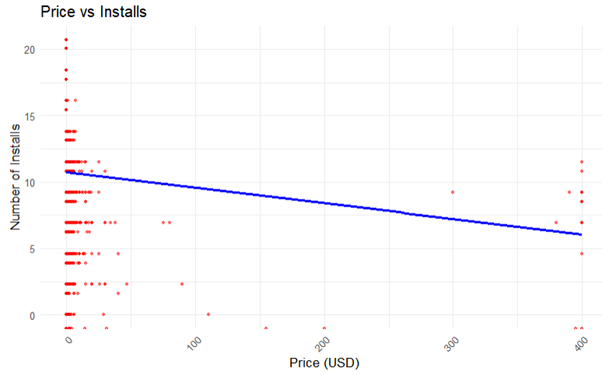
\includegraphics{installs_vs_price.png}

Figure 1 reveals that the majority of app installs are concentrated in
free apps, with a notable decline as app prices increase. This
illustrates a strong inverse relationship between price and installs,
emphasizing consumer preference for free options over paid ones in the
app market.

\textbf{Figure 2}. Scatterplot for Correlation Between Days Since Last
Update and Rating

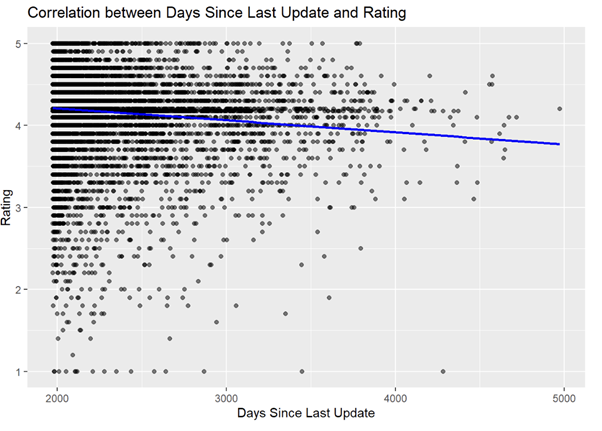
\includegraphics{rating_vs_days_since_update.png}

In Figure 2, it can be observed that as the number of days since the
last update increase, app ratings tend to decline. This trend showcases
the critical role of regular updates in maintaining user satisfaction
and app quality.

\textbf{Figure 3}. Boxplot for Installs vs.~Update Category for Each
Content Rating

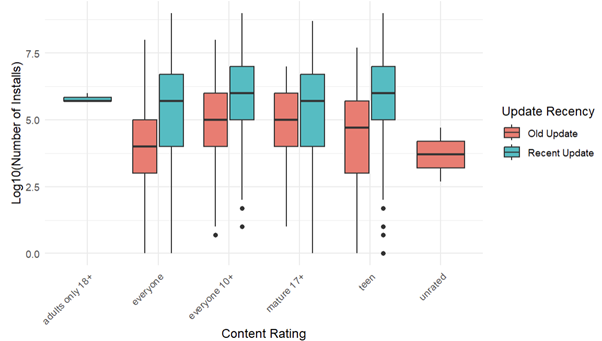
\includegraphics{installs_vs_update_vs_content_rating.png}

Figure 3 reveals a notable difference in installs between apps with
recent and old updates. Apps with recent updates tend to have higher
install rates compared to those with older updates. Additionally, apps
rated for ``Everyone 10+'' have the highest number of installs among the
different content ratings.

\textbf{Figure 4}. Plot for Installs vs.~Size

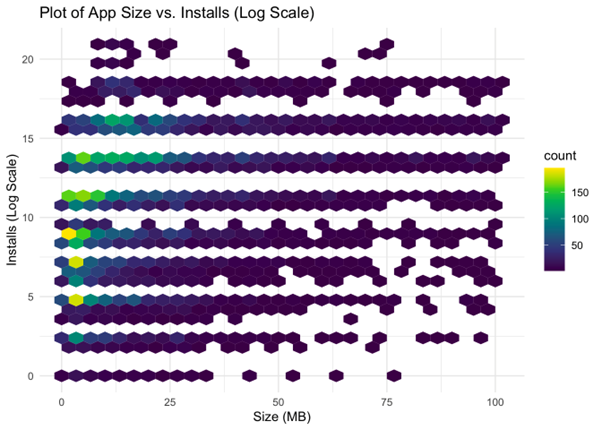
\includegraphics{installs_vs_size.png}

In Figure 4, there is no strong, linear relationship between app size
and install count. The data points are scattered across the plot,
indicating that app size does not necessarily determine the number of
installs.

\textbf{Figure 5}. Plot for Installs vs.~Rating

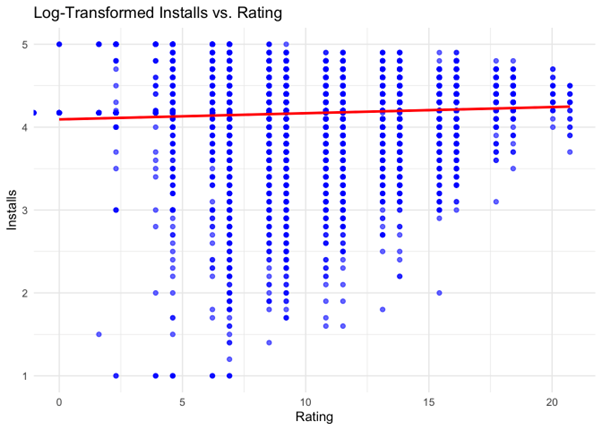
\includegraphics{installs_vs_rating.png}

Figure 5 suggests a slight positive correlation between app rating and
install count. Apps with higher ratings tend to have higher install
numbers, especially in the higher rating ranges. However, the
relationship is not perfectly linear, and other factors likely influence
install counts.

\textbf{Figure 6}. Plot for Mean Rating by Review Category

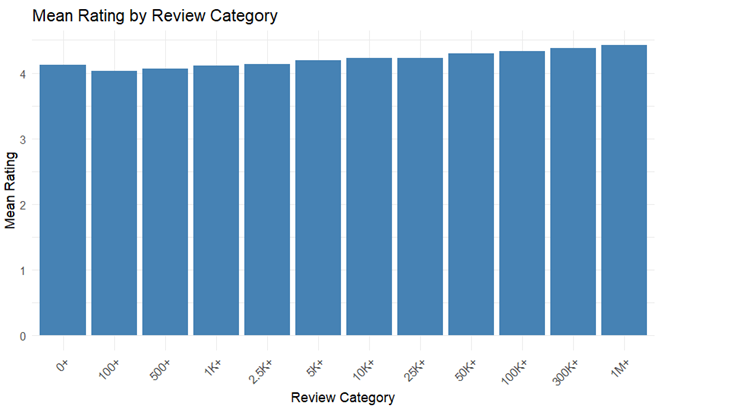
\includegraphics{review_vs_rating.png}

Figure 6 indicates a positive correlation between review count and
rating. This suggests that apps with a higher number of reviews tend to
have higher ratings. This trend implies that a larger number of reviews
can positively influence an app's overall rating.

\textbf{Figure 7}. Scatterplot for Installs vs.~Reviews

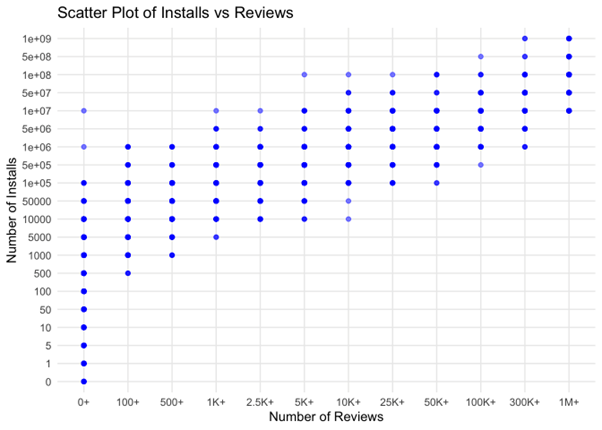
\includegraphics{installs_vs_review.png}

Figure 7 reveals a positive correlation between review category and
install count. Apps with higher review categories, likely indicating a
larger number of positive reviews, tend to have higher install numbers.
This finding reinforces the trend observed in Figure 6, where higher
ratings are associated with higher installs.

\textbf{Figure 8}. Boxplot for Top 5 Category with Most Installs

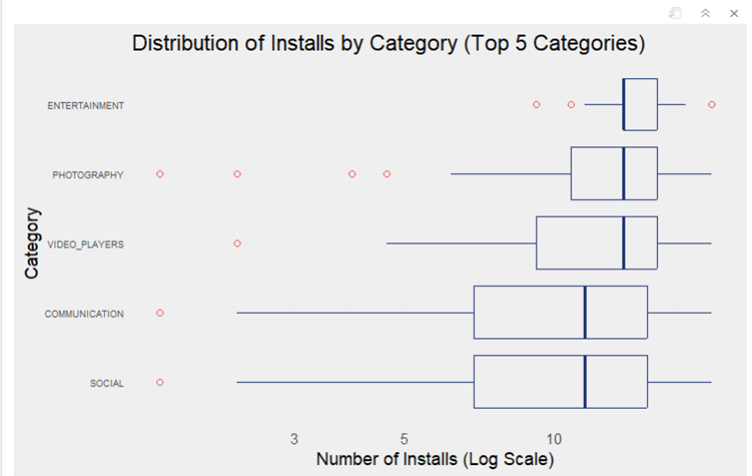
\includegraphics{top_5_cat.png}

In Figure 8, it is evident that the top five categories with the highest
number of installs are Entertainment, Photography, Video, Communication,
and Social. This suggests that applications like WhatsApp and Messenger
rank among the most installed, aligning with their daily use by many
users. The popularity of these categories reflects a trend where apps
enhancing social interaction and visual expression dominate user
preferences, contributing to high engagement rates.

\textbf{Figure 9}. Heatmap for Correlations Between the Variables

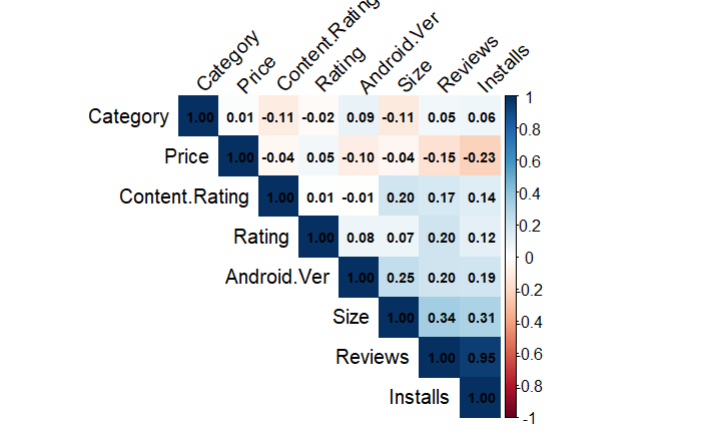
\includegraphics{correlation.png}

In Figure 9, several key correlations can be observed:

Strong Correlation (i). \textbf{Installs and Reviews}: - A very strong
positive correlation of \textbf{0.95} indicates that apps with more
installs tend to receive more reviews. This suggests that popular apps
attract significant user feedback.

Moderate Correlation (ii). \textbf{Price and Installs}: - A negative
correlation of \textbf{-0.23} suggests that higher-priced apps generally
have fewer installs compared to free apps. (iii). \textbf{Size and
Installs}: - A positive correlation of \textbf{0.31} indicates that
larger apps tend to have higher installs, although this may also reflect
specific categories that have larger app sizes. (iv). \textbf{Days Since
Last Update and Installs}: - A negative correlation of \textbf{-0.33}
implies that older updates are associated with fewer installs,
highlighting the importance of regular updates in attracting users.

Slight Correlation (v). \textbf{Reviews and Ratings}: - There is a
slight correlation suggesting that higher ratings are associated with
more reviews, indicating that positive feedback may lead to increased
user engagement. (vi). \textbf{Android Version and Installs}: -
Compatibility with more Android versions is positively correlated with
higher installs, suggesting that broader compatibility may enhance an
app's reach.

These observations underscore significant relationships between app
characteristics and user engagement metrics, offering valuable insights
for developers and marketers.While the relationships between installs,
reviews, and ratings provide valuable insights, it suggests that
focusing solely on install counts could suffice for assessing an app's
popularity. This perspective emphasizes the significance of installs as
a primary metric, potentially simplifying the evaluation process for
developers and marketers.

\section{\texorpdfstring{\textbf{SMART
Question}}{SMART Question}}\label{smart-question}

``What is the impact of content rating, required Android version, app
category, size, and pricing on predicting app success in terms of
positive ratings and high user reviews, as well as the number of
installs, using data from Google Play Store apps from 2010 to 2018?''

\subsubsection{SMART Analysis}\label{smart-analysis}

The proposed research question investigates how various factors---such
as content rating, required Android version, app category, size, and
pricing---affect the success of applications on the Google Play Store,
specifically in terms of positive ratings, high user reviews, and
download numbers. By analyzing data from 2010 to 2018, this study aims
to identify patterns and correlations that could provide insights into
what drives user engagement and satisfaction. Understanding these
relationships will be critical for developers seeking to enhance app
performance and appeal in a competitive market.

\subsubsection{Probing Smart Question: Hypothesis Testing
Approach}\label{probing-smart-question-hypothesis-testing-approach}

Our research aims to answer the following questions:

\textbf{\emph{Question 1: Does price significantly impact the popularity
of an app in terms of installs?}}

\begin{itemize}
\item
  \textbf{Null Hypothesis (H₀):} There is no significant difference in
  the mean log installs between free and paid apps. (Price does not
  impact app popularity.)
\item
  \textbf{Alternate Hypothesis (H₁):} There is a significant difference
  in the mean log installs between free and paid apps. (Price impacts
  app popularity.)
\item
  \textbf{Test:} Independent t-test t-value: 29.042 Degrees of Freedom
  (df): 977.19 P-value: \textless{} 2.2e-16
\item
  \textbf{Observation:} The p-value is extremely small (less than 0.05),
  which indicates strong evidence against the null hypothesis. The mean
  log installs for free apps (11.002709) is significantly higher than
  for paid apps (7.284829).
\item
  \textbf{Conclusion:} Since the p-value is very small, we reject the
  null hypothesis and conclude that the difference in mean log installs
  between free and paid apps is statistically significant. This suggests
  that price does indeed have a significant impact on app popularity in
  terms of installs.
\end{itemize}

\textbf{\emph{Question 2: Does Reviews and Ratings have significantly
impact the popularity of an app in terms of installs?}}

\begin{itemize}
\item
  \textbf{Null Hypothesis (H₀):} There is no significant difference in
  the mean rating across different review categories. (Review count does
  not impact app rating.)
\item
  \textbf{Alternate Hypothesis (H₁):} There is a significant difference
  in the mean rating across different review categories. (Review count
  impacts app rating.)
\item
  \textbf{Test:} ANOVA F Value (f): 41.3 Degrees of Freedom (df): 11
  P-value: \textless{} 2e-16
\item
  \textbf{Observation:} The p-value is extremely small (less than 0.05),
  indicating strong evidence against the null hypothesis. The mean
  rating generally increases with higher review categories, from 4.03 in
  the ``100+'' category to 4.43 in the ``1M+'' category.
\item
  \textbf{Conclusion:} Since the p-value is very small, we reject the
  null hypothesis. This suggests that the number of reviews does have a
  statistically significant impact on the mean rating. Higher-rated
  apps, particularly those with many reviews, are likely more popular,
  indicating that review count and rating significantly impact app
  popularity in terms of installs.
\end{itemize}

\textbf{\emph{Question 3: Does Update have significant impact on
Rating?}}

\begin{itemize}
\item
  \textbf{Null Hypothesis (H₀):}The number of days since the last update
  does not significantly impact the app rating.
\item
  \textbf{Alternate Hypothesis (H₁):} The number of days since the last
  update does significantly impact the app rating.
\item
  \textbf{Test:} ANOVA (Analysis of Variance) F-value: 143.8 P-value:
  \textless{} 2e-16
\item
  \textbf{Observation:} The p-value is extremely small (less than 0.05),
  indicating strong evidence against the null hypothesis. A high F-value
  (143.8) further supports that there is a significant difference in app
  ratings based on the time since the last update.
\item
  \textbf{Conclusion:} Since the p-value is very small, we reject the
  null hypothesis and conclude that the time since the last update has a
  statistically significant impact on app ratings.
\end{itemize}

\textbf{\emph{Question 4: Does Content Rating and Last Updated
significantly impact the popularity of an app in terms of installs?}}

\begin{itemize}
\item
  \textbf{Null Hypothesis (H₀):} There is no significant difference in
  the mean log installs between apps with different content ratings.
  (Content Rating does not impact app popularity.)
\item
  \textbf{Alternate Hypothesis (H₁):} There is a significant difference
  in the mean log installs between apps with different content ratings.
  (Content Rating impacts app popularity.)
\item
  \textbf{Test:} ANOVA F-Value: 41.95 Degrees of Freedom (df): 5, 9638
  P-value: \textless{} 2e-16
\item
  \textbf{Observation:} The p-value is extremely small (less than 0.05),
  indicating strong evidence against the null hypothesis.The ANOVA
  results suggest a significant difference in installs between content
  ratings, implying that content rating categories have an impact on the
  number of installs.
\item
  \textbf{Conclusion:} Since the p-value is very small, we reject the
  null hypothesis and conclude that the difference in installs between
  content ratings is statistically significant. This suggests that
  content rating does indeed have a significant impact on app popularity
  in terms of installs.
\end{itemize}

\textbf{\emph{Question 5: Does app size have significant impact on the
number of Installs ?}}

\begin{itemize}
\item
  \textbf{Null Hypothesis (H₀):} There is no significant correlation
  between app size and the number of installs. (App size does not impact
  the number of installs.)
\item
  \textbf{Alternate Hypothesis (H₁):} There is a significant correlation
  between app size and the number of installs. (App size impacts the
  number of installs.) Test:
\item
  \textbf{Test}: Correlation t-test t-value: 4.0069 Degrees of Freedom
  (df): 9657 P-value: 6.198e-05 Correlation Coefficient: 0.0407 95\%
  Confidence Interval: 0.0208 to 0.0606
\item
  \textbf{Observation:} The p-value is very small (less than 0.05),
  indicating strong evidence against the null hypothesis.However, the
  correlation coefficient (0.0407) is close to zero, suggesting a weak
  positive correlation between app size and the number of installs.
\item
  \textbf{Conclusion:} Since the p-value is very small, we reject the
  null hypothesis, concluding that there is a statistically significant
  but weak positive correlation between app size and the number of
  installs. This suggests that app size has a minor impact on the number
  of installs.
\end{itemize}

\section{\texorpdfstring{\textbf{Conclusion}}{Conclusion}}\label{conclusion}

Expanding on the insights drawn from the analysis of Google Play Store
applications, this study dives deep into the intricate factors that
influence an app's success, particularly concerning the number of
installations and user ratings. The Google Play Store, as a massive
platform hosting millions of applications across various categories,
provides a unique landscape to explore how specific attributes correlate
with app popularity and user engagement. This comprehensive conclusion
will not only reflect the observed patterns and associations among
variables such as content rating, app size, update frequency, and
pricing but also emphasize the broader implications of these findings on
app development, user engagement, and market strategy.

\textbf{1. Content Rating as a Key Indicator of User Trust and
Accessibility}

One of the most significant findings in this study is the strong
influence of content rating on app installations and user ratings.
Content rating serves as a proxy for the target audience's age group,
indicating whether an app is suitable for all ages or is intended for a
specific demographic, such as teenagers or adults. Apps rated for
general audiences often tend to have higher installation rates, largely
due to their broader accessibility. On the other hand, apps with mature
content or restricted ratings may appeal to a narrower, more specific
audience.

The impact of content rating can be understood through user psychology
and trust. Users tend to favor applications that are considered safe and
suitable for their age group or for a wider range of age groups, leading
to higher installation rates for apps with general ratings. Developers
who understand this correlation can leverage it to design applications
that meet the needs of a diverse audience. For example, a gaming app
with engaging, family-friendly content is likely to appeal to both
children and adults, potentially increasing its reach and popularity. In
contrast, apps targeted solely at adults might focus more on niche
functionality, understanding that they may attract fewer installs but
potentially more engaged users.

\textbf{2. The Role of Update Frequency in Sustaining User Engagement}

Another critical aspect that emerged from the analysis is the positive
correlation between update frequency and app success, as seen through
both installations and user ratings. Apps that are frequently updated
tend to maintain a higher level of user engagement by addressing bugs,
introducing new features, and aligning with the latest technological
advancements. Users appreciate apps that evolve, as it shows that
developers are invested in improving the user experience. Consequently,
apps with regular updates often receive better ratings, as users
recognize the developer's commitment to quality and enhancement.

The strategic significance of this insight lies in the maintenance and
continuous improvement of apps. For instance, developers working on a
utility app, like a calendar or weather app, may find that incorporating
user feedback into regular updates improves user retention and
satisfaction. Conversely, an app that remains stagnant is more likely to
lose users to competitors who consistently innovate and respond to user
demands. This finding suggests that app developers should adopt a
proactive approach, utilizing user feedback to guide updates and
optimize the app's performance and features continually.

\textbf{3. App Size and Performance Trade-offs}

App size, while a statistically significant factor, exhibited a
relatively weaker correlation with installations compared to other
variables. The size of an app can influence its download rate,
especially in regions where data limitations or lower-end devices with
limited storage capacity are common. However, as mobile device storage
capacities have increased, this factor may hold less weight in more
developed regions or among users with high-end devices. Nevertheless,
developers should be cautious about app size, particularly for users
with restricted data plans or older devices.

From a strategic perspective, balancing functionality with size becomes
crucial. An app overloaded with features may provide a comprehensive
experience but may be less attractive if it requires substantial
storage. For example, a photo-editing app might gain popularity if it
offers high-quality features within a compact size. Developers can adopt
techniques such as data compression, modular design, or cloud
integration to reduce app size, making their apps accessible to a
broader user base. This consideration reflects a growing need in the app
market to create high-functioning but lightweight applications that
cater to all user groups, regardless of their device specifications.

\textbf{4. Pricing Models and Consumer Preferences}

One of the most pronounced findings of this study is the preference for
free applications, which enjoy higher installation rates than paid
counterparts. The modern app marketplace reflects a significant consumer
bias towards free apps, likely driven by the vast number of alternative
options available at no cost. For developers, this insight has profound
implications for app monetization strategies. While a paid model might
initially seem advantageous for revenue generation, it could deter a
large segment of potential users who are unwilling to pay upfront.

The preference for free apps suggests that developers may benefit from
exploring alternative monetization strategies, such as in-app
advertisements, freemium models, or in-app purchases. A freemium model,
for instance, allows users to access the core functionalities of an app
for free while offering additional premium features for a fee. This
model has proven successful for many applications, as it provides a path
for revenue generation without limiting user reach. An alternative is
in-app advertising, where developers can generate income through
advertisements displayed within the app. However, developers should be
mindful of user experience, as overly intrusive ads may lead to negative
ratings and decreased user retention.

\textbf{5. Implications for App Developers and Market Strategies}

This study provides developers and marketers with actionable insights
into optimizing app offerings for the Google Play Store, emphasizing the
need for a user-centric approach in app design and strategy. By
understanding the variables that contribute to app success, developers
can make informed decisions on where to focus their resources and how to
structure their product features. For instance, creating an app that is
accessible to all audiences (as indicated by content rating),
lightweight, frequently updated, and free to install could significantly
enhance an app's chances of success in the competitive app market.

Furthermore, this analysis highlights the importance of adopting a
data-driven approach to app development. By analyzing patterns in user
feedback and behaviors, developers can prioritize updates that address
prevalent issues or add popular features, thus enhancing user
satisfaction and increasing the likelihood of positive ratings and
recommendations. Such a strategy is particularly vital in the current
competitive landscape, where user loyalty is often contingent on
seamless, reliable, and up-to-date experiences.

\textbf{6. Limitations and Future Research Directions}

While this analysis offers valuable insights, it is essential to
acknowledge its limitations and suggest areas for future research. The
study primarily focused on a subset of variables and did not account for
other potential factors, such as app category, regional trends, or
cultural preferences, which could influence user behavior. Future
studies could expand on these findings by examining additional data
sources or utilizing a larger dataset. Additionally, it would be
beneficial to explore the causal relationships among variables, such as
whether frequent updates directly cause higher ratings or if
highly-rated apps are more likely to receive updates. Exploring these
nuances could yield even more targeted insights for developers.

In conclusion, this study of Google Play Store applications underscores
the importance of key factors like content rating, update frequency, app
size, and pricing in determining app success. By aligning their
strategies with these findings, developers can enhance their app's
appeal, foster positive user engagement, and maintain competitive
standing. As the app market continues to grow, staying informed of these
trends will be crucial for developers seeking long-term success in an
increasingly dynamic and competitive environment.

\section{\texorpdfstring{\textbf{References}}{References}}\label{references}

Brandom, R. (2019, May 7). There are now 2.5 billion active Android
devices. The Verge.
\url{https://www.theverge.com/2019/5/7/18528297/google-io-2019-android-devices-play-store-total-number-statistic-keynote}

faisaljanjua0555. (2023a, May 20). eda - google play store apps. Kaggle.
\url{https://www.kaggle.com/code/faisaljanjua0555/eda-google-play-store-apps/input}

Fischer, F., \& Kleen, S. (2021). Possibilities, Problems, and
Perspectives of Data Collection by Mobile Apps in Longitudinal
Epidemiological Studies: Scoping Review. Journal of medical Internet
research, 23(1), e17691. \url{https://doi.org/10.2196/17691}

Paula, D. F. O. de, Menezes, B. H. X. M., \& Araújo, C. C. (1970,
January 1). Building a quality mobile application: A user-centered study
focusing on design thinking, user experience and usability.
SpringerLink.
\url{https://link.springer.com/chapter/10.1007/978-3-319-07626-3_29\#citeas}

\end{document}
